\section{First-order Reduction of the ADM Evolution Equations in 3+1 Dimensions with Spherical Symmetry}
\label{sec:adm}

Finally, we will solve the ADM evolution equations in 3+1 dimensions with spherical symmetry, reduced to first order (equation \eqref{eq:ADM}). For this, we will be providing the initial conditions

\begin{align}
    \begin{array}{@{}l@{}}
        A(0,x) = 0.002 e^{-2.0 x^2}+1,
        \\
        B(0,x) = 0.002 e^{-2.0 x^2}+1,
        \\
        D_A(0,x) = - \frac{0.008 x e^{-2.0 x^2}}{1 + 0.002 e^{-2.0 x^2}},
        \\
        D_B(0,x) = - \frac{0.008 x e^{-2.0 x^2}}{1 + 0.002 e^{-2.0 x^2}},
        \\
        K_A(0,x) = 0,
        \\
        K_B(0,x) = 0,
        \\
        \lambda(0,x) = 0,
        \\
        \alpha(0,x) = 1,
        \\
        D_\alpha (0,x) = 0.
    \end{array}
    \label{eq:GR_IC}
\end{align}

We will be considering a system of length $L = 10$, imposing that $A$, $B$, $K_A$, and $K_B$ are even functions, that $D_A$, $D_B$, and $\lambda$ are odd functions, and forcing the solution to not evolve at "infinity". Just like before, this treatment at the right-most boundary is not sensible. However, like before, the boundary is sufficiently far away to not compromise the solution. Naturally, we will use artificial dissipation, with a dissipation coefficient of $\sigma = 0.02$.%%

We will be solving these equations with resolutions of 500, 1000, 2000, 4000, and 8000 points, which we, again, combine in pairs twice and use the nomenclature previously introduced.

The norm convergence of the results for $A$ can be found in figure \ref{fig:norm_A}, while the pointwise convergence of the $A$ and $K_A$ for $x = 0$ (up to $t = 0.75$, since the error grows too rapidly for the analysis of the graph to be possible from that point on) are found in figures \ref{fig:point_A} and \ref{fig:point_KA}. The respective graphs for $B$ and $K_B$ are very similar to their counterparts $A$ and $K_A$ when it comes to pointwise error, so they are found in the appendix, together with the graphs for the auxiliary quantities $D_A$, $D_B$, and $\lambda$. The norm convergence between all the fields is also very similar, so the rest of them are also found in the appendix.

\begin{figure}[t!]
    \centering
    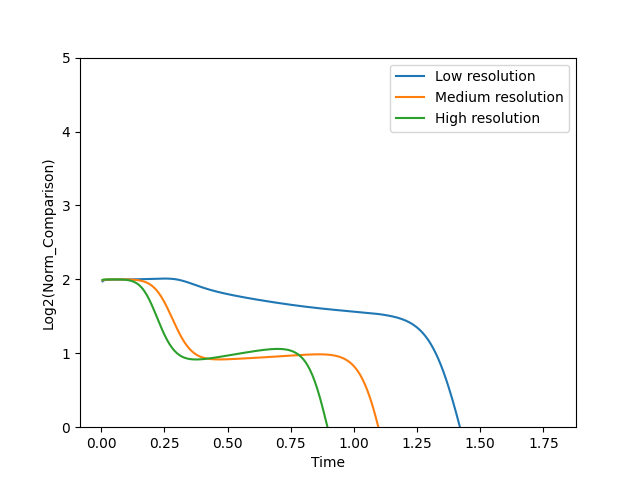
\includegraphics[width=\columnwidth]{Images/A-norm.png}
    \caption{Norm convergence of the evolution of $A$ (with artificial dissipation $\sigma = 0.02$) while imposing the parity of the fields at the origin and not evolving "infinity", giving initial conditions represented in equation \eqref{eq:GR_IC}}
    \label{fig:norm_A}
\end{figure}

\begin{figure}[t!]
    \centering
    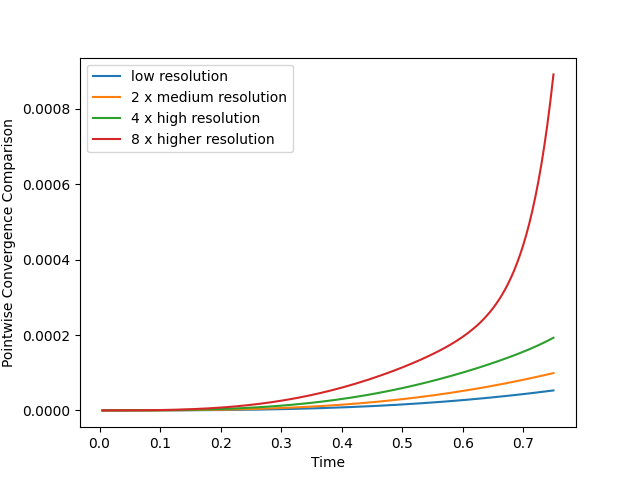
\includegraphics[width=\columnwidth]{Images/A-point.png}
    \caption{Pointwise convergence at position $x = 0$ of the evolution of $A$ (with artificial dissipation $\sigma = 0.02$) while imposing the parity of the fields at the origin and not evolving "infinity", giving initial conditions represented in equation \eqref{eq:GR_IC}}
    \label{fig:point_A}
\end{figure}

\begin{figure}[t!]
    \centering
    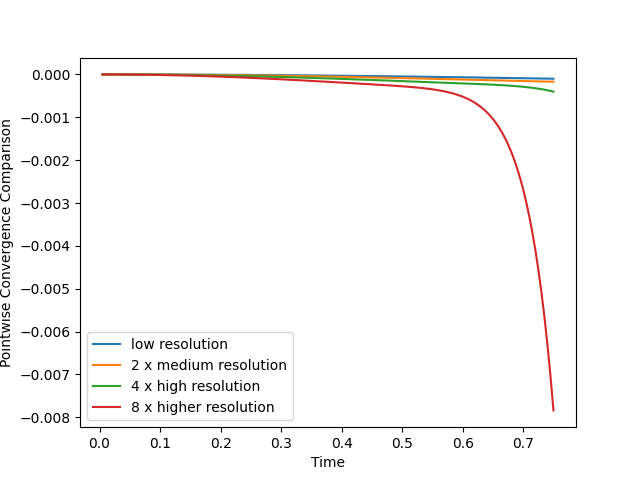
\includegraphics[width=\columnwidth]{Images/KA-point.png}
    \caption{Pointwise convergence at position $x = 0$ of the evolution of $K_A$ (with artificial dissipation $\sigma = 0.02$) while imposing the parity of the fields at the origin and not evolving "infinity", giving initial conditions represented in equation \eqref{eq:GR_IC}}
    \label{fig:point_KA}
\end{figure}

The intensity plots for $A$, $B$, $K_A$ and $K_B$ are found in figures \ref{fig:A}, \ref{fig:B}, \ref{fig:KA} and \ref{fig:KB} respectively.

\begin{figure}[t!]
    \centering
    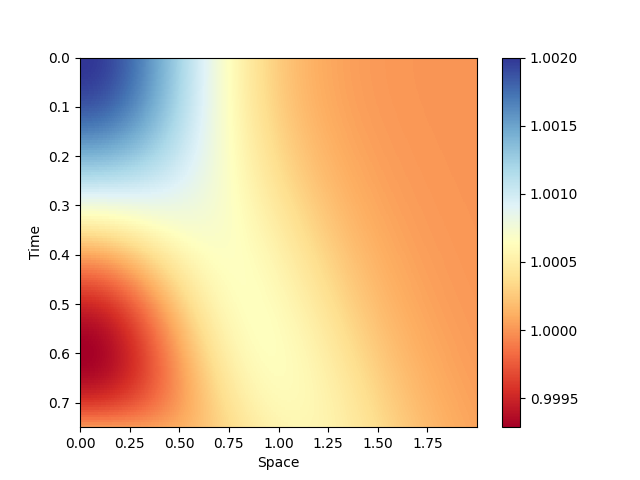
\includegraphics[width=\columnwidth]{Images/adm_evolution-2nd_order-A.png}
    \caption{Intensity plot of the evolution of $A$ (with artificial dissipation $\sigma = 0.02$) while imposing the parity of the fields at the origin and not evolving "infinity", giving initial conditions represented in equation \eqref{eq:GR_IC}}
    \label{fig:A}
\end{figure}

\begin{figure}[t!]
    \centering
    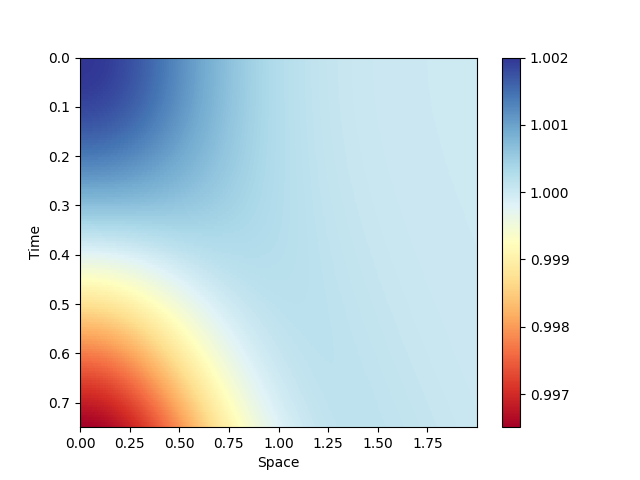
\includegraphics[width=\columnwidth]{Images/adm_evolution-2nd_order-B.png}
    \caption{Intensity plot of the evolution of $B$ (with artificial dissipation $\sigma = 0.02$) while imposing the parity of the fields at the origin and not evolving "infinity", giving initial conditions represented in equation \eqref{eq:GR_IC}}
    \label{fig:B}
\end{figure}

\begin{figure}[t!]
    \centering
    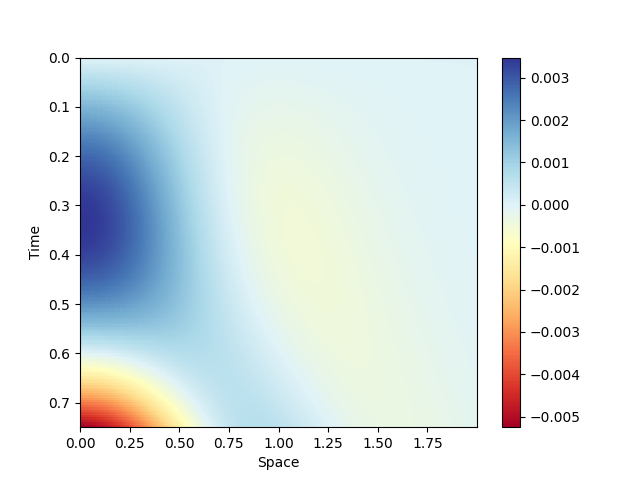
\includegraphics[width=\columnwidth]{Images/adm_evolution-2nd_order-KA.png}
    \caption{Intensity plot of the evolution of $K_A$ (with artificial dissipation $\sigma = 0.02$) while imposing the parity of the fields at the origin and not evolving "infinity", giving initial conditions represented in equation \eqref{eq:GR_IC}}
    \label{fig:KA}
\end{figure}

\begin{figure}[t!]
    \centering
    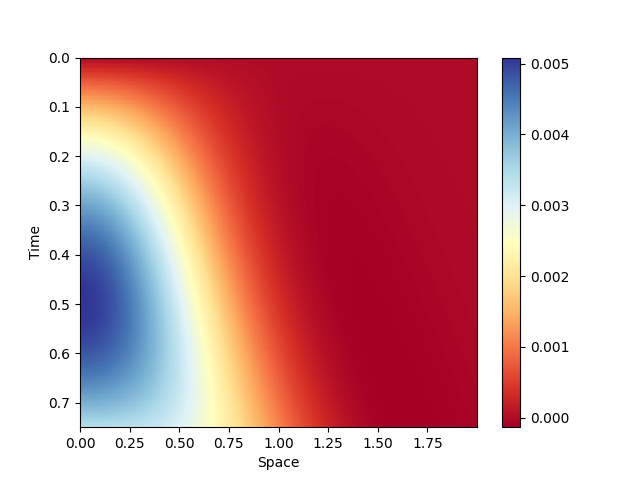
\includegraphics[width=\columnwidth]{Images/adm_evolution-2nd_order-KB.png}
    \caption{Intensity plot of the evolution of $K_B$ (with artificial dissipation $\sigma = 0.02$) while imposing the parity of the fields at the origin and not evolving "infinity", giving initial conditions represented in equation \eqref{eq:GR_IC}}
    \label{fig:KB}
\end{figure}

The results show that our code seems to be functional for slight time evolution. After that, $A$ and $B$, and $K_A$ and $K_B$ start to drift apart at the origin, where they should coincide. We can check the validity of our solutions by looking at the momentum and Hamiltonian constraints in figures \ref{fig:momentum} and \ref{fig:hamiltonian}. We could also look at the reduction constraints, however they don't seem to be violated, so they are found in the appendix.

\begin{figure}[t!]
    \centering
    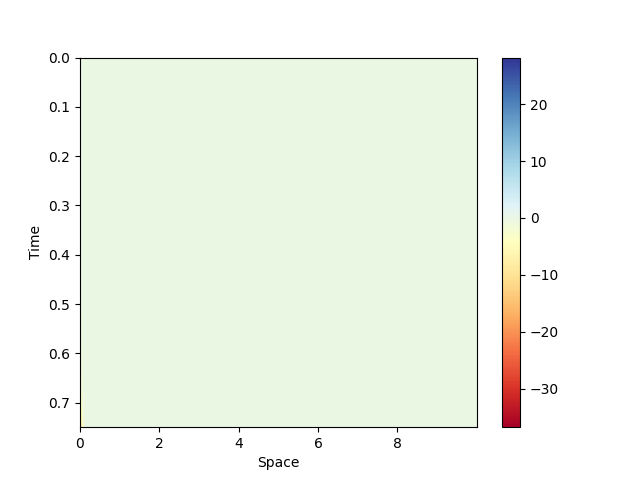
\includegraphics[width=\columnwidth]{Images/adm_evolution-2nd_order-Momentum.png}
    \caption{Intensity plot of the momentum constraint of the evolution, where we imposed the parity of the fields at the origin and have not evolved "infinity", giving initial conditions represented in equation \eqref{eq:GR_IC}}
    \label{fig:momentum}
\end{figure}

\begin{figure}[t!]
    \centering
    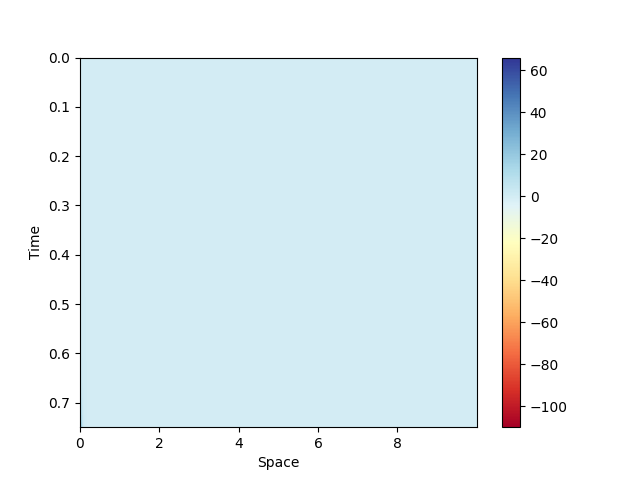
\includegraphics[width=\columnwidth]{Images/adm_evolution-2nd_order-Hamiltonian.png}
    \caption{Intensity plot of the Hamiltonian constraint of the evolution, where we imposed the parity of the fields at the origin and have not evolved "infinity", giving initial conditions represented in equation \eqref{eq:GR_IC}}
    \label{fig:hamiltonian}
\end{figure}

Even though it is not possible to see in these figures, even though the value of the constraints is practically zero everywhere, that is not true for the origin, where they are violated. This indicates that we are not treating the origin properly, and should try to correct that.

However, this correction was not possible in the time frame of this project. It happens that our problem is not well posed, as we are using geodesic slicing, and combining that with our coordinate choice, it is guaranteed to make coordinate singularities in finite time. Because of that, in order to make our code correct, we would have to reformulate our problem and develop completely new code for the solution of the ADM evolution equations.